% System Analysis and Design: Inventory Management System (StockPilot)
% Compile with: pdflatex system-design.tex   (run twice for the table of contents)
% The diagrams are in the diagrams/ folder. To rebuild a diagram:
%   use-case:   cd diagrams && pdflatex use-case.tex
%   activity:   dot -Tpdf activity-sale.dot -o activity-sale.pdf  (same for activity-purchase)
%   class / ER: python3 gen_class.py && dot -Tpdf class-diagram.dot -o class-diagram.pdf
%               python3 gen_er.py    && dot -Tpdf er-diagram.dot -o er-diagram.pdf
\documentclass[11pt,a4paper]{article}
\usepackage[T1]{fontenc}
\usepackage{lmodern}
\usepackage[margin=2.5cm]{geometry}
\usepackage{graphicx}
\usepackage{booktabs}
\usepackage{tabularx}
\usepackage{array}
\newcolumntype{Y}{>{\raggedright\arraybackslash}X}
\newcolumntype{P}[1]{>{\raggedright\arraybackslash}p{#1}}
\usepackage{enumitem}
\usepackage{pdflscape}
\usepackage{float}
\usepackage{fancyhdr}
\usepackage{xcolor}
\usepackage[hidelinks]{hyperref}
\hypersetup{colorlinks=true, linkcolor=blue, urlcolor=blue}

\pagestyle{fancy}
\fancyhf{}
\fancyhead[L]{Inventory Management System}
\fancyhead[R]{System Analysis and Design}
\fancyfoot[C]{\thepage}
\renewcommand{\headrulewidth}{0.4pt}
\setlength{\parskip}{0.35em}
\setlist{itemsep=0.15em, topsep=0.3em}

\newcommand{\code}[1]{\texttt{#1}}

\begin{document}

\begin{titlepage}
  \centering
  \vspace*{3cm}
  {\LARGE\bfseries Inventory Management System\par}
  \vspace{0.4cm}
  {\Large Using MERN Stack\par}
  \vspace{1.5cm}
  {\Large\bfseries Step 1: System Analysis and Design\par}
  \vspace{0.4cm}
  {\large Scenarios, Use Case Diagram, Activity Diagrams,\\ Class Diagram and Database Diagram\par}
  \vfill
  {\large Web Engineering Lab Project\par}
  \vspace{0.3cm}
  {\large Jashore University of Science and Technology\par}
  \vspace{2cm}
\end{titlepage}

\tableofcontents
\newpage

\section{Introduction}
This document presents the analysis and design of the \textbf{Inventory Management System}
described in the project proposal. It contains the usage scenarios, the use case diagram,
two activity diagrams (sales and purchase), the class diagram and the database diagram.

The system follows a \textbf{Client--Server--Database} architecture: a React.js client
calls RESTful APIs of a Node.js and Express.js server, which stores data in MongoDB.
Access is controlled with JWT authentication and three roles:
\textbf{Administrator}, \textbf{Manager} and \textbf{Staff}.

\section{Scenarios}
A scenario describes one realistic situation, step by step, from the user's point of view.
The scenarios below cover the main business flows of the system.

\subsection{Scenario 1: Walk-in sale}
\textbf{Actor:} Staff.\quad \textbf{Precondition:} the staff user is logged in; the product is in stock.
\begin{enumerate}
  \item A customer without an account wants to buy two Bluetooth speakers and pay in cash.
  \item The staff user opens \emph{New sale}, leaves the customer empty (walk-in) and selects \emph{Cash}.
  \item The staff user searches the product by name, enters quantity 2 and creates a draft sale.
  \item The system takes the price from the product record and saves the sale as \code{DRAFT}.
  \item The staff user presses \emph{Complete}. The system checks the stock, reduces it by 2,
        writes a stock movement and records the full payment.
  \item The staff user prints the invoice and gives it to the customer.
\end{enumerate}
\textbf{Result:} the sale is \code{COMPLETED} and \code{PAID}; the stock and its history are updated.

\subsection{Scenario 2: Credit sale with partial payment}
\textbf{Actor:} Staff.\quad \textbf{Precondition:} the customer is registered.
\begin{enumerate}
  \item A regular customer buys a laptop worth 90,000 but pays only 50,000 now.
  \item The staff user creates and completes the sale with the customer selected.
        The sale becomes \code{UNPAID} with 90,000 outstanding.
  \item The staff user collects a payment of 50,000 by mobile banking with the transaction ID as reference.
  \item The system saves the payment and changes the status to \code{PARTIALLY\_PAID} with 40,000 outstanding.
  \item Later, the Manager opens \emph{Payments and Dues} and sees the customer's due.
\end{enumerate}
\textbf{Result:} the due is tracked against a named customer; a payment can never exceed the outstanding amount.

\subsection{Scenario 3: Purchase from a supplier and supplier payment}
\textbf{Actor:} Manager.\quad \textbf{Precondition:} the supplier and products exist.
\begin{enumerate}
  \item The shop orders 10 speakers from a supplier. The Manager creates a draft purchase;
        the unit price is filled from the product's purchase price and can be changed.
  \item When the goods arrive, the Manager checks them and presses \emph{Complete}.
        The system increases the stock by 10 and writes a \code{PURCHASE} stock movement.
  \item The Manager pays part of the bill by bank transfer using \emph{Pay supplier}.
  \item The purchase shows \emph{Partly paid}; \emph{Payments and Dues} shows how much is still owed to the supplier.
\end{enumerate}
\textbf{Result:} stock, purchase total and supplier dues are all correct. A draft can be cancelled
without touching stock; a completed purchase cannot be cancelled.

\subsection{Scenario 4: Damaged product and low-stock alert}
\textbf{Actor:} Manager.
\begin{enumerate}
  \item During a stock count, one keyboard is found broken.
  \item The Manager opens \emph{Inventory}, chooses \emph{Adjust stock}, type \emph{Damaged / lost},
        quantity 1 and writes a reason.
  \item The system reduces the stock (never below zero) and writes the movement with the reason and user.
  \item The stock is now at the minimum level, so the product appears in the low-stock alert on the dashboard.
\end{enumerate}

\subsection{Scenario 5: Customer return, and cancelling a wrong return}
\textbf{Actor:} Manager.
\begin{enumerate}
  \item A customer returns one item from an unpaid sale. The Manager records a customer return
        with a reason. Stock increases and the customer's balance is reduced by the item's value.
  \item The Manager notices the return was saved against the wrong sale and cancels it with a reason.
  \item In one transaction the system takes the item out of stock again, restores the balance
        and marks the return \code{CANCELLED} (the record is kept).
\end{enumerate}
\textbf{Note:} a return that already handed cash back to the customer cannot be cancelled.

\subsection{Scenario 6: Administrator adds a staff user}
\textbf{Actor:} Administrator.
\begin{enumerate}
  \item A new salesperson joins. The Administrator creates a user with the \code{STAFF} role and a temporary password.
  \item At the first login the new user must change the password.
  \item The staff user can sell and add customers, but cannot see purchases, reports, user management or the audit log.
  \item Every important action is written to the audit log, which only the Administrator can view.
\end{enumerate}

\section{Use Case Diagram}
Figure~\ref{fig:usecase} shows what each role can do. The roles form a hierarchy:
a Manager can do everything a Staff user can, and an Administrator can do everything a Manager can.
The diagram follows the role checks that the server applies on every API request.

\begin{figure}[H]
  \centering
  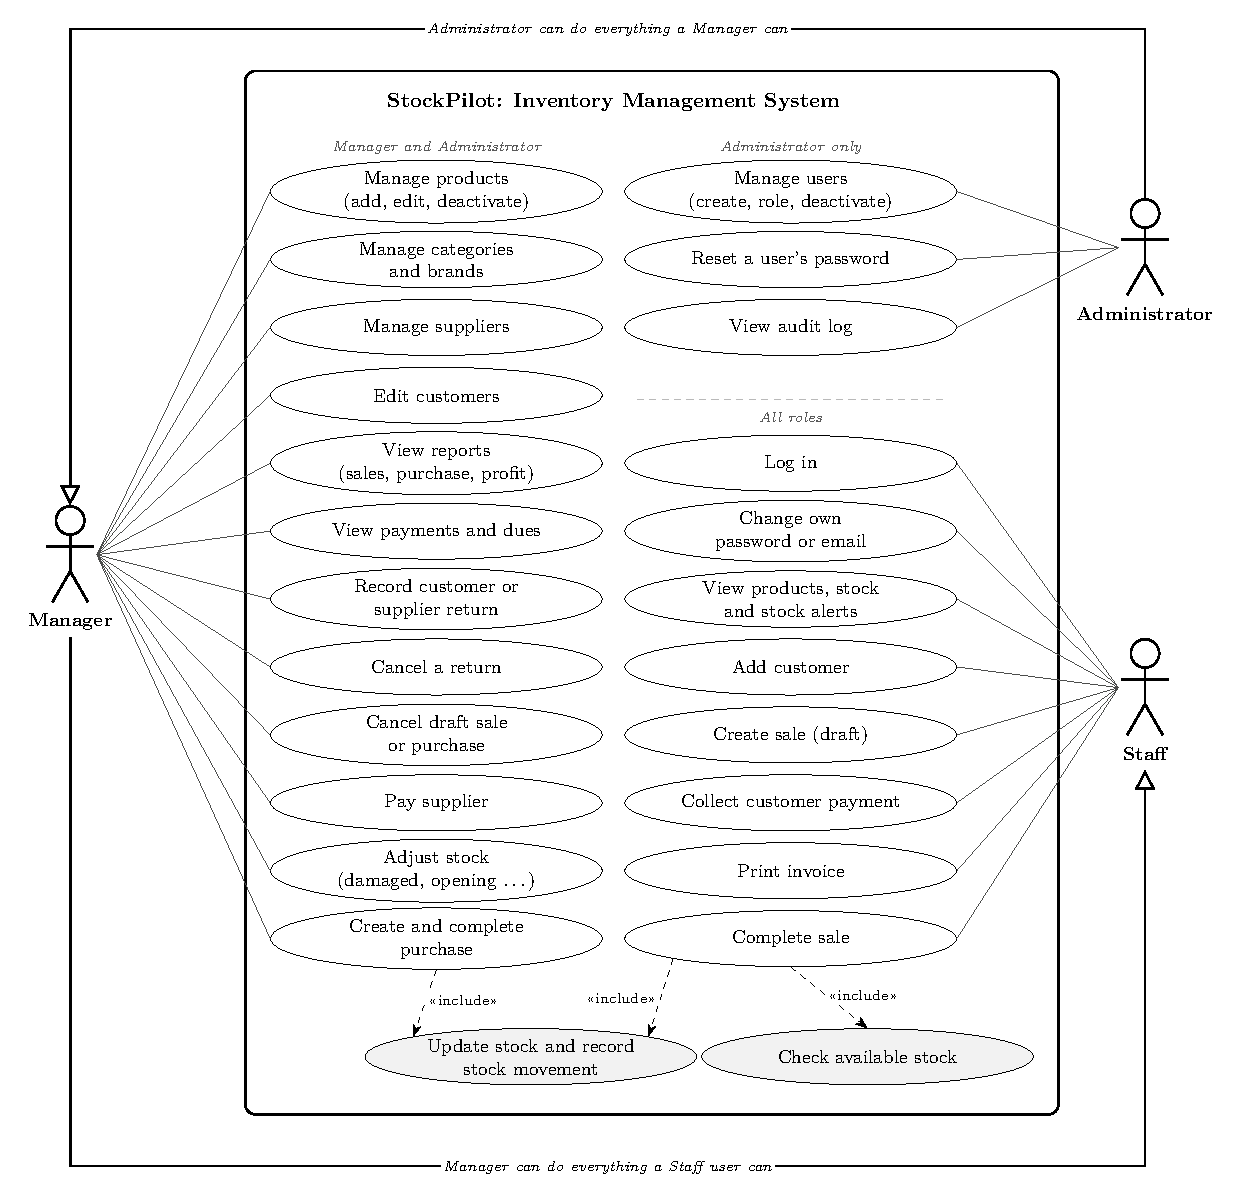
\includegraphics[width=\textwidth]{diagrams/use-case.pdf}
  \caption{Use case diagram}
  \label{fig:usecase}
\end{figure}

\begin{table}[H]
  \centering
  \caption{Actors and their responsibilities}
  \begin{tabularx}{\textwidth}{@{}lY@{}}
    \toprule
    \textbf{Actor} & \textbf{Responsibilities} \\
    \midrule
    Staff & Log in, view products and stock, create and complete sales, collect customer payments,
            print invoices and add customers. \\
    Manager & All Staff tasks, plus products, categories, brands, suppliers, purchases, supplier payments,
              stock adjustment, returns, cancelling drafts and returns, reports, and payments and dues. \\
    Administrator & All Manager tasks, plus user management (create, role, deactivate, reset password)
                    and the audit log. \\
    \bottomrule
  \end{tabularx}
\end{table}

\section{Activity Diagrams}
The activity diagrams show the two most important business processes. The left lane shows
what the user does and the right lane shows what the system does. The dashed box marks the steps
that run inside one MongoDB transaction: either all of them are saved, or none of them.

\subsection{Sales process}
A sale is first saved as a draft. When it is completed, the system checks the stock of every item.
If any item does not have enough stock, the whole transaction is rolled back. A walk-in customer pays
the full amount at completion; a named customer can pay later in parts.

\begin{figure}[H]
  \centering
  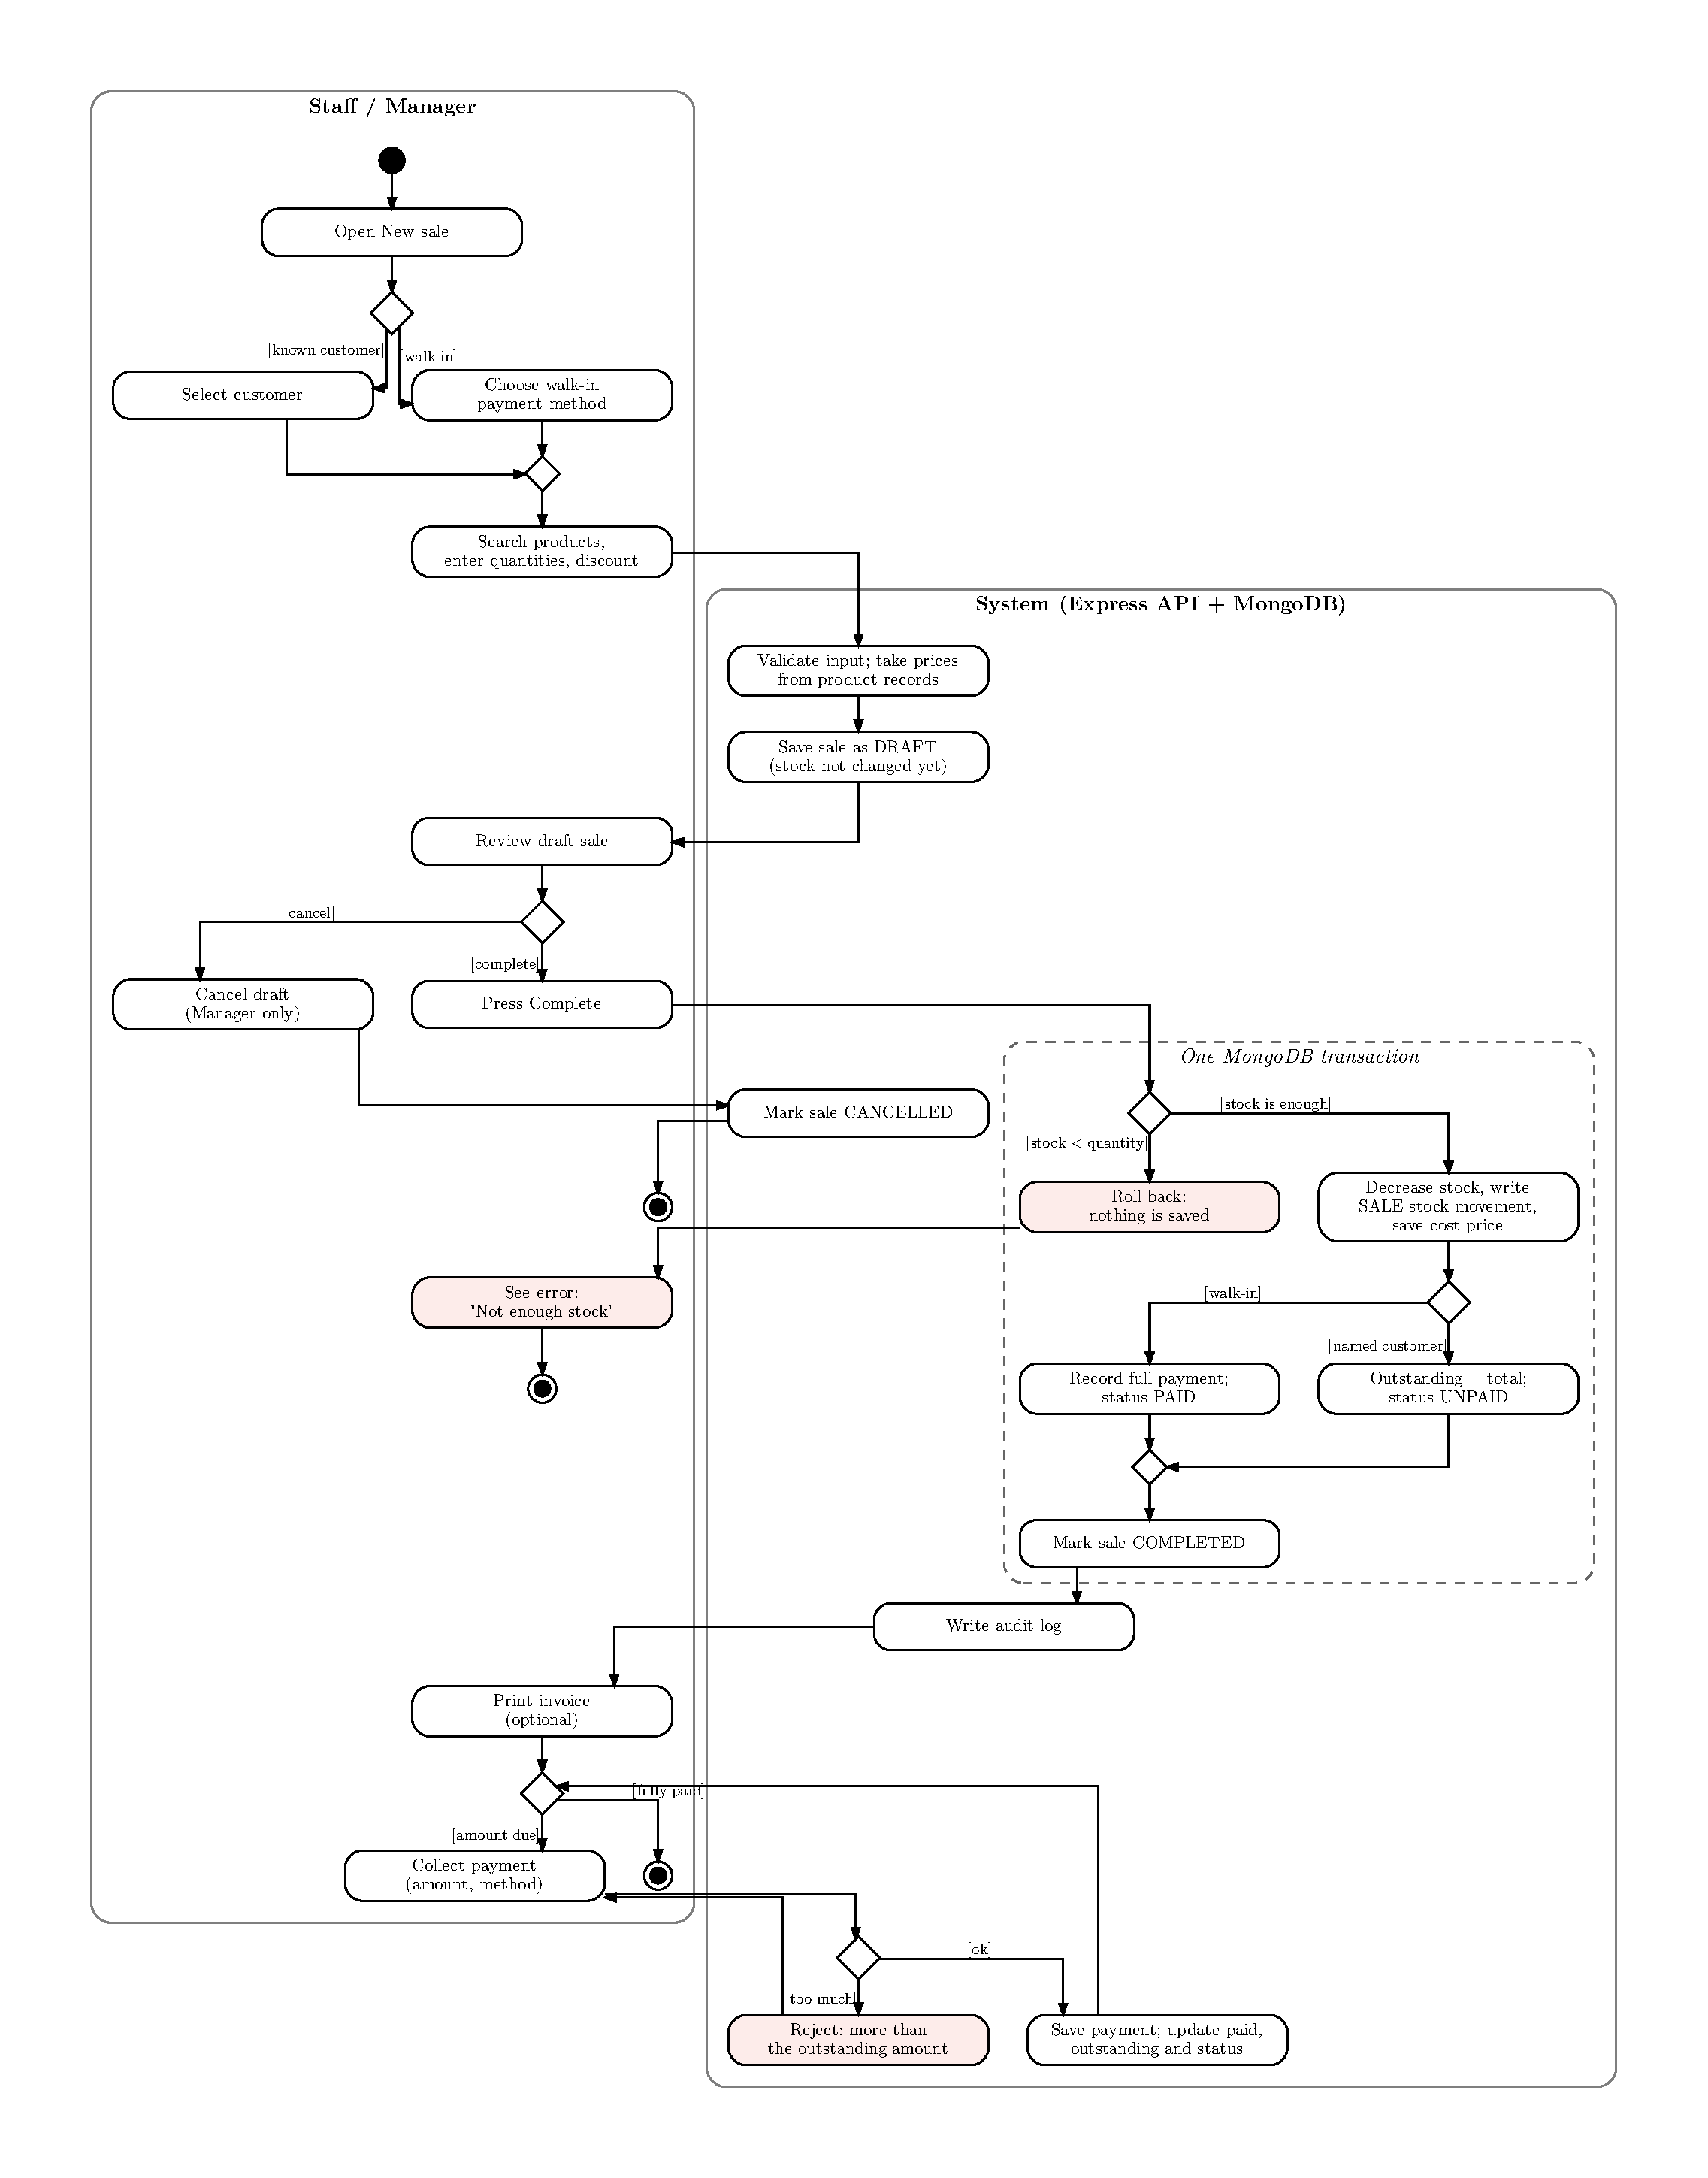
\includegraphics[width=\textwidth,height=0.78\textheight,keepaspectratio]{diagrams/activity-sale.pdf}
  \caption{Activity diagram: sales process}
  \label{fig:activity-sale}
\end{figure}

\subsection{Purchase process}
A purchase is also a draft first. Completing it increases the stock and writes the stock history in one
transaction. Payments to the supplier can be made at once or later, and can never exceed what is still owed
(bill minus returned goods minus payments already made).

\begin{figure}[H]
  \centering
  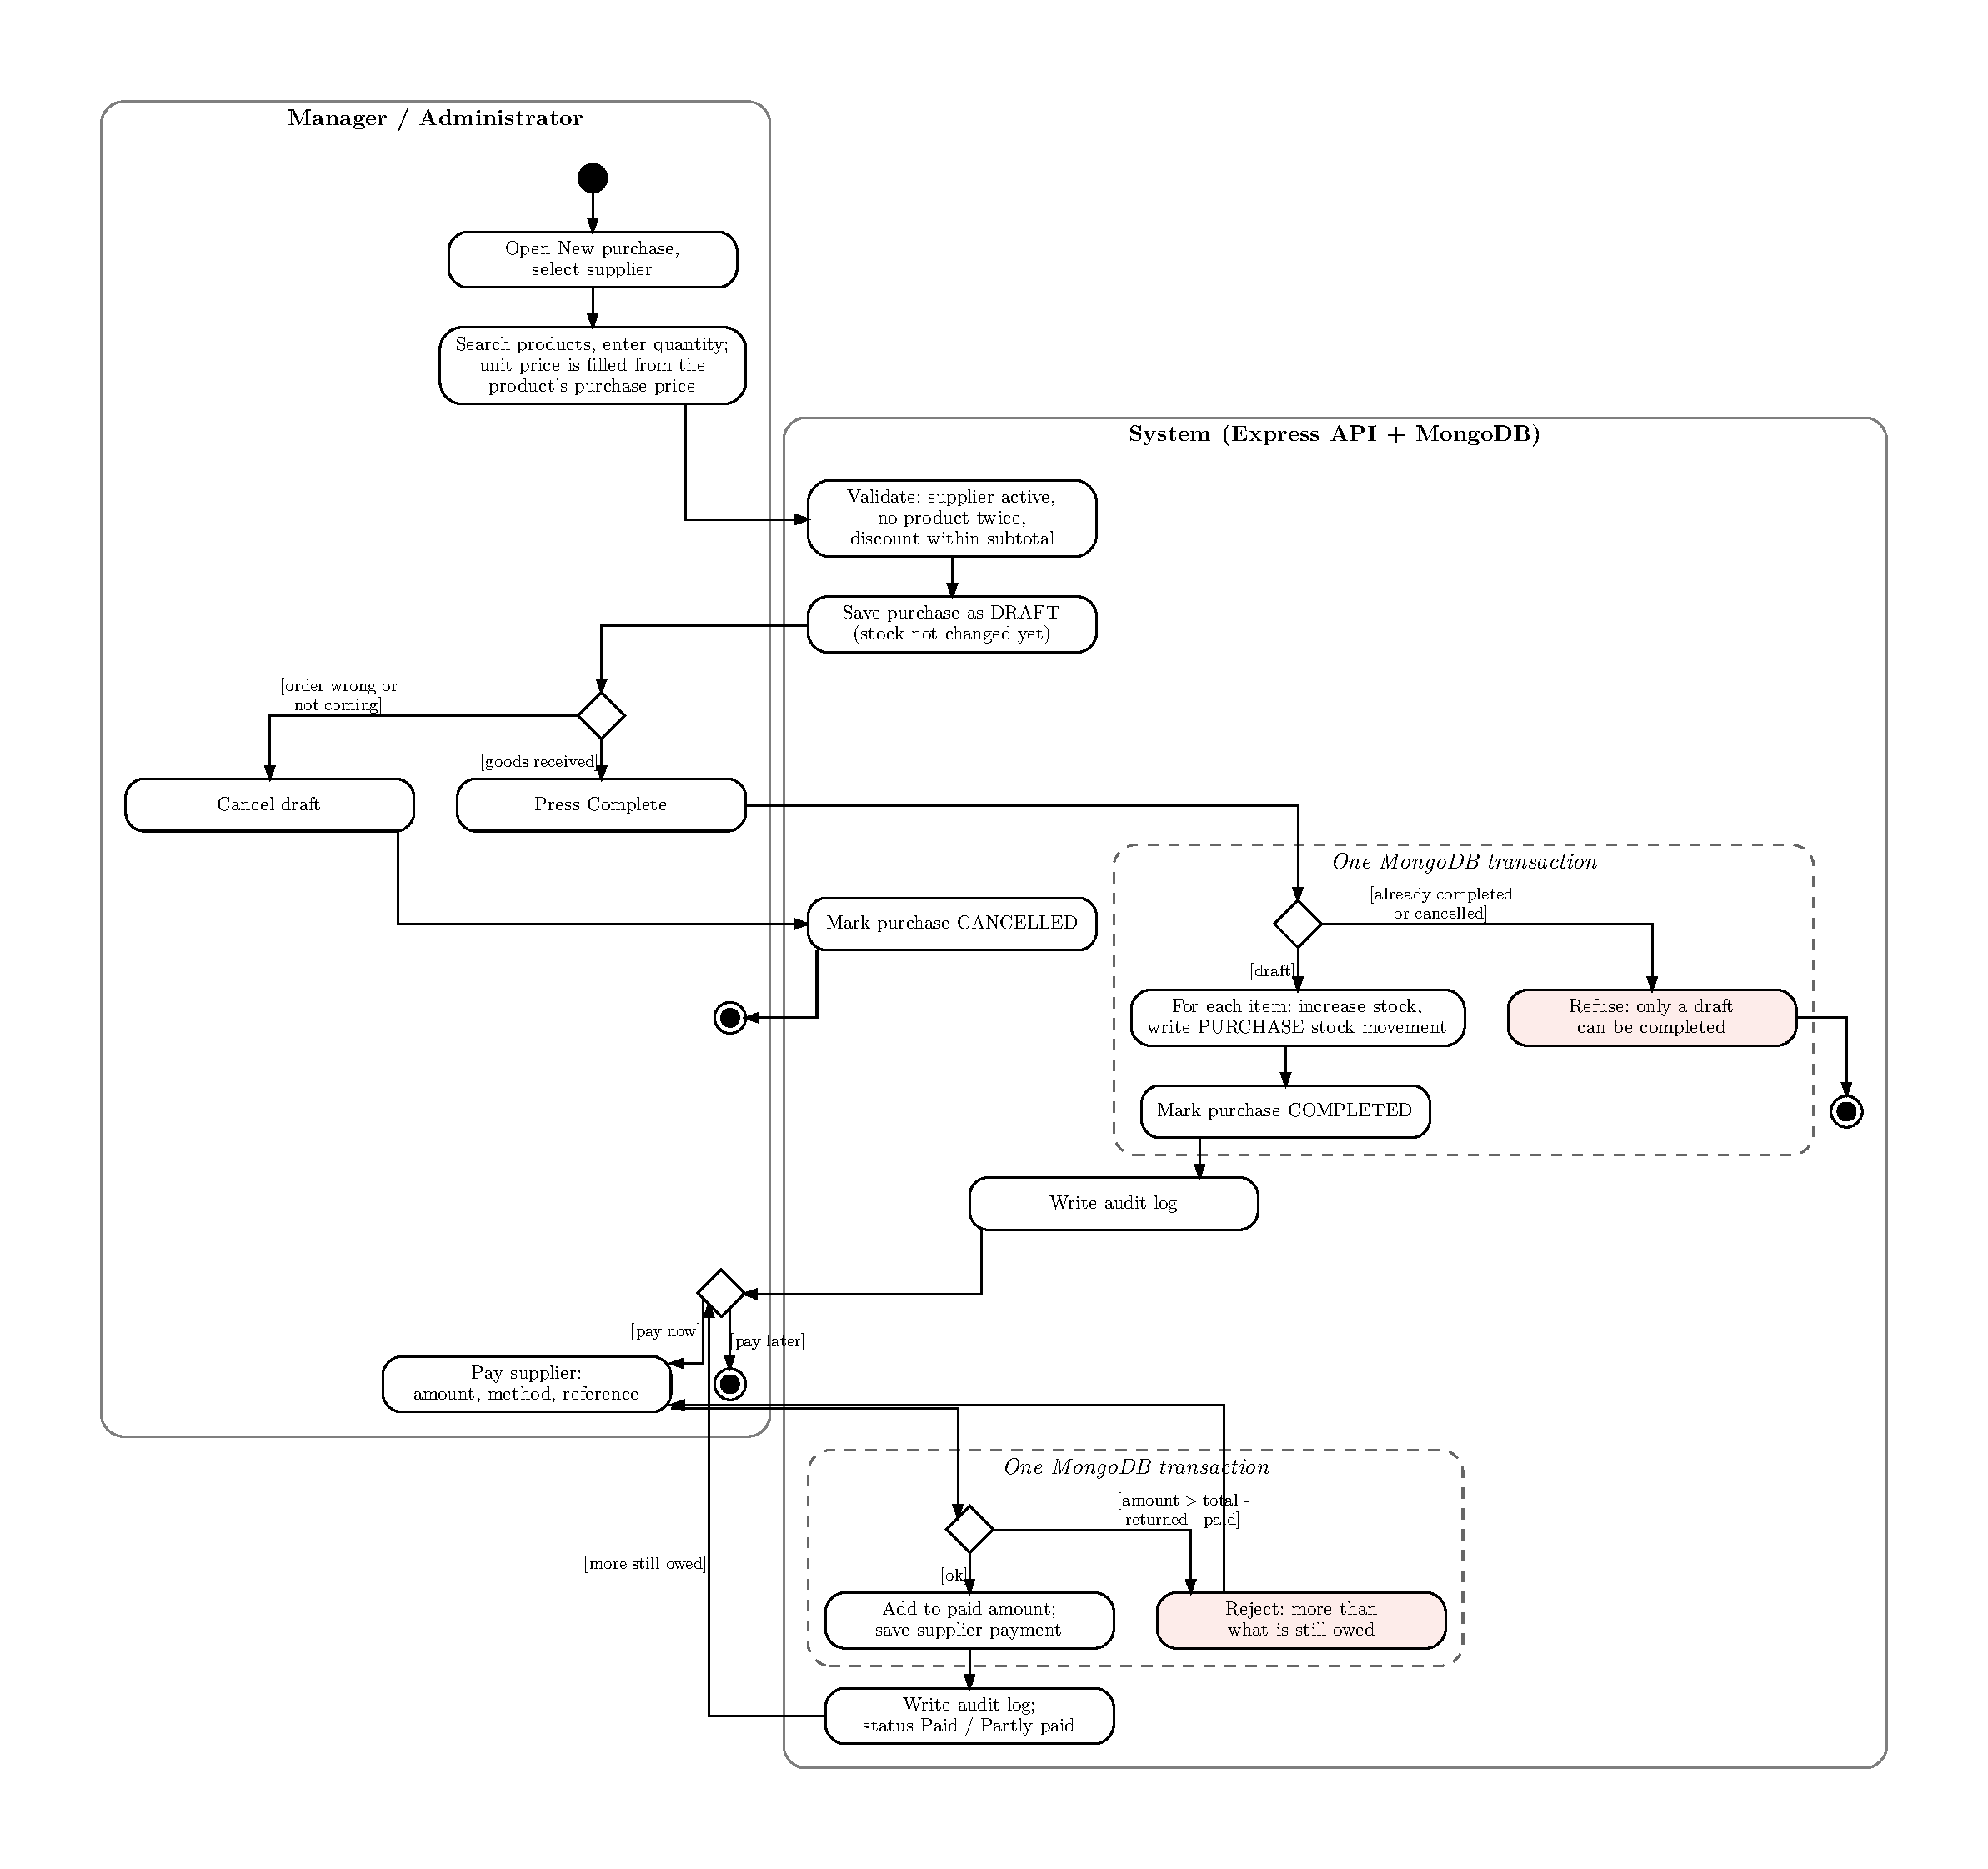
\includegraphics[width=\textwidth,height=0.78\textheight,keepaspectratio]{diagrams/activity-purchase.pdf}
  \caption{Activity diagram: purchase process}
  \label{fig:activity-purchase}
\end{figure}

\clearpage
\section{Class Diagram}
Each class is a Mongoose model in \code{server/src/models}. Sale, purchase and return lines are
\emph{embedded documents} (filled diamond = composition): they are stored inside their parent
document and cannot exist alone. Enumerations list the allowed values of status and type fields.

\begin{figure}[H]
  \centering
  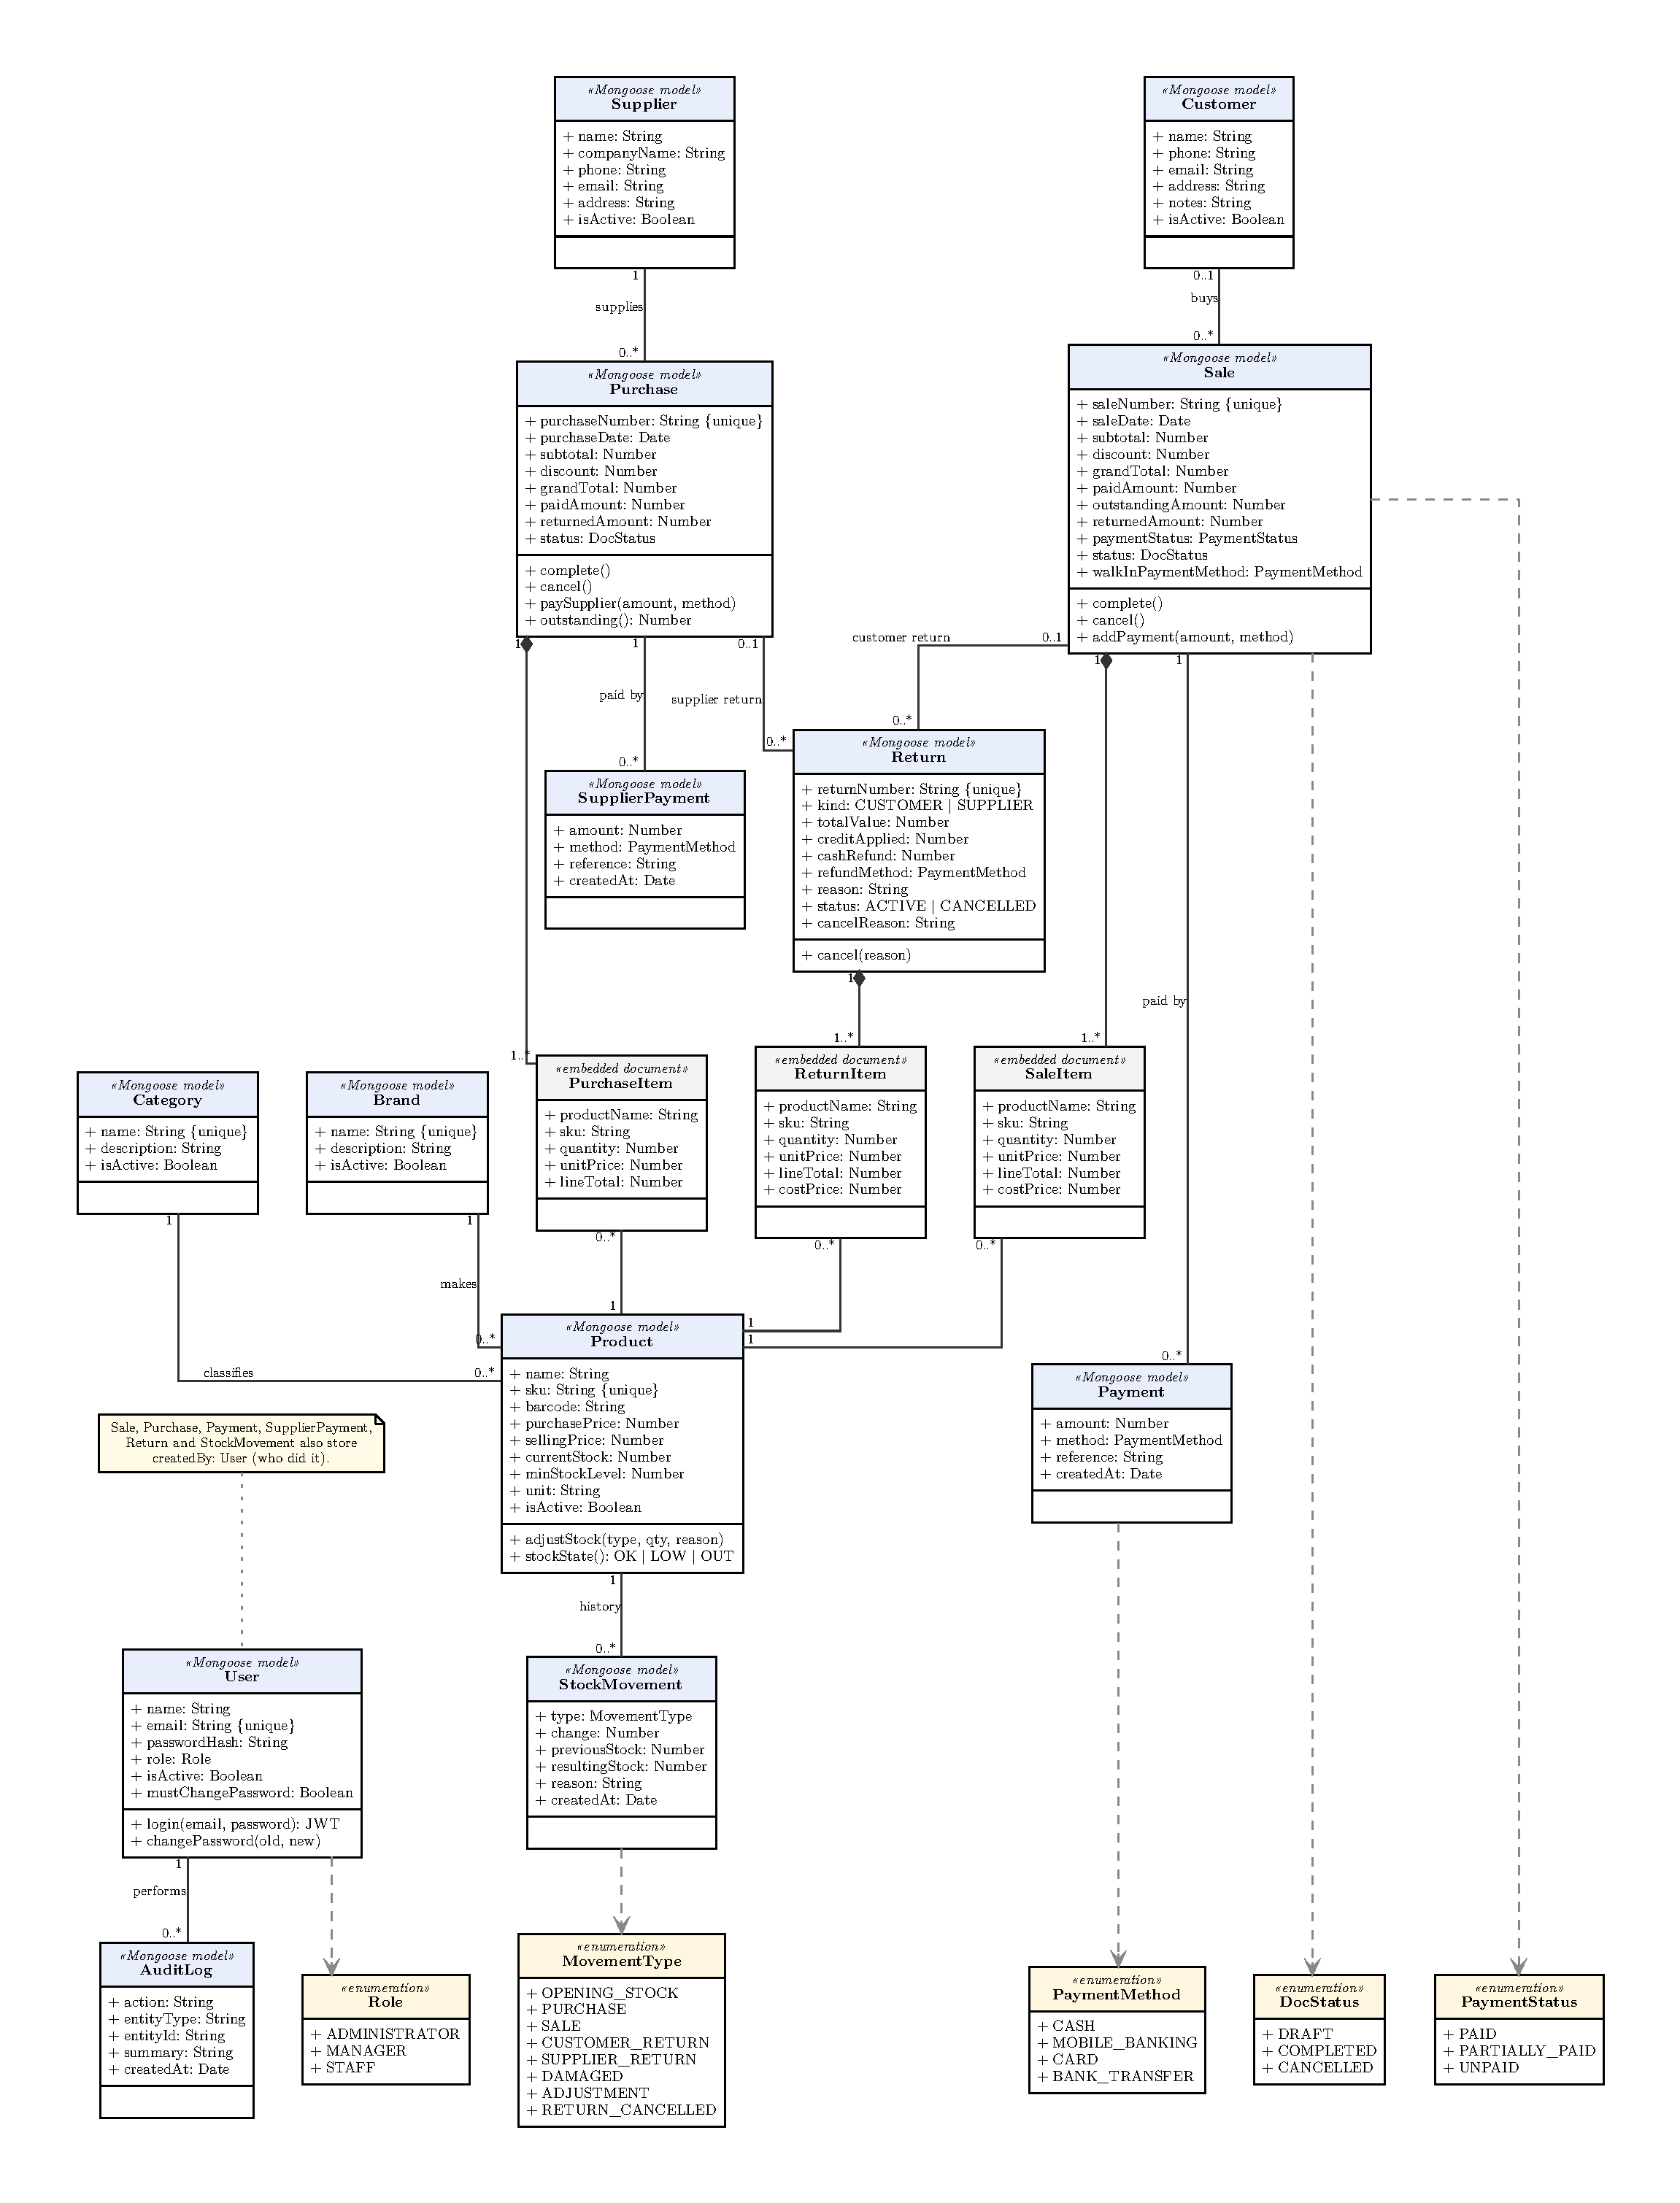
\includegraphics[width=\textwidth,height=0.8\textheight,keepaspectratio]{diagrams/class-diagram.pdf}
  \caption{Class diagram}
  \label{fig:class}
\end{figure}

\clearpage
\section{Database Diagram}
The database is MongoDB with 13 collections. References between collections are stored as
\code{ObjectId} values (FK). Line items are embedded inside sales, purchases and returns, so one
document holds a whole bill and can be read in one query.

\begin{figure}[H]
  \centering
  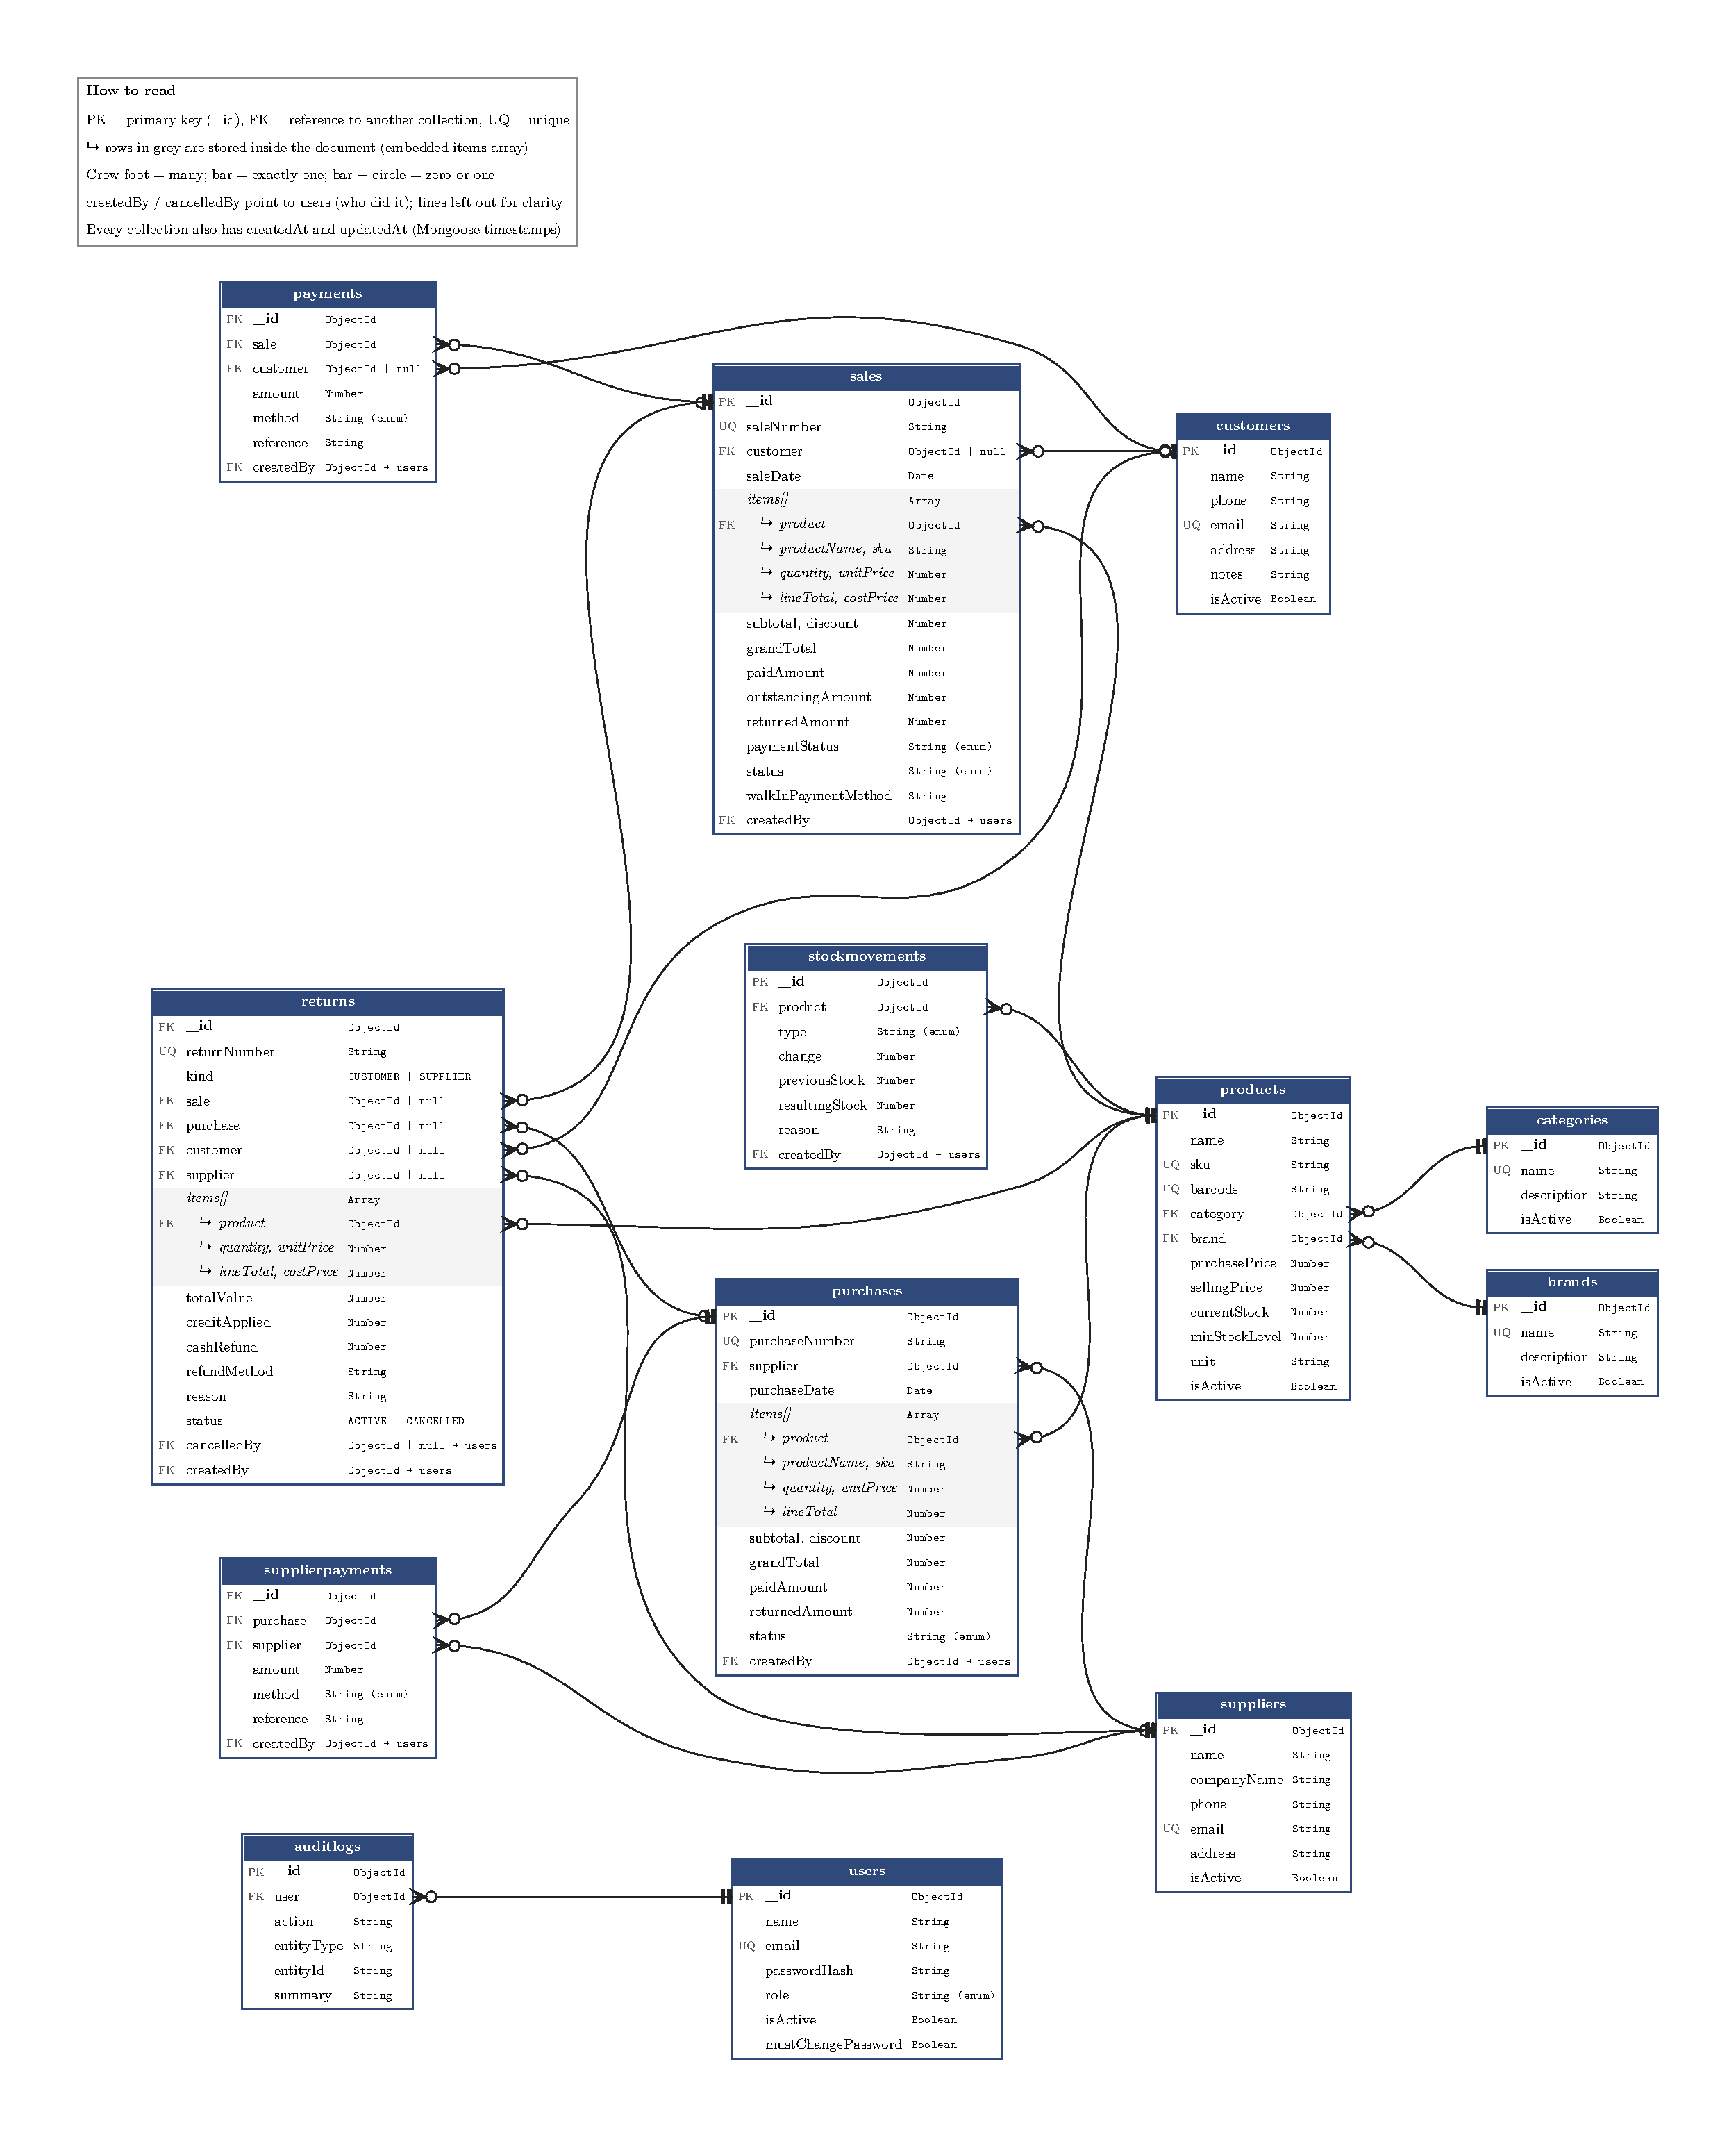
\includegraphics[width=\textwidth,height=0.8\textheight,keepaspectratio]{diagrams/er-diagram.pdf}
  \caption{Database (ER) diagram of the MongoDB collections}
  \label{fig:er}
\end{figure}

\begin{table}[H]
  \centering
  \caption{Collections}
  \begin{tabularx}{\textwidth}{@{}lY@{}}
    \toprule
    \textbf{Collection} & \textbf{Stores} \\
    \midrule
    users & System users, hashed passwords and roles \\
    categories, brands & Product classification \\
    products & Products, SKU, barcode, prices, current stock, minimum stock level \\
    customers, suppliers & Business partners \\
    purchases & Purchase bills with embedded items, paid and returned amounts \\
    sales & Sales bills with embedded items, cost price per line, payment status \\
    payments & Money received from customers for sales \\
    supplierpayments & Money paid to suppliers for purchases \\
    returns & Customer and supplier returns with embedded items; can be cancelled \\
    stockmovements & Every stock change with type, before and after quantity, reason and user \\
    auditlogs & Who did what and when \\
    \bottomrule
  \end{tabularx}
\end{table}

\section{Design Changes from the Proposal}
The design was refined while building the system, as the proposal allowed
(\emph{``The final database schema and relationships will be refined during the system design phase''}).

\begin{table}[H]
  \centering
  \caption{Proposal compared with the final design}
  \begin{tabularx}{\textwidth}{@{}P{2.7cm}P{4.4cm}Y@{}}
    \toprule
    \textbf{Topic} & \textbf{Proposal} & \textbf{Final design and reason} \\
    \midrule
    Roles & Separate \code{roles} collection & A \code{role} field on \code{users} with three fixed values.
      The roles never change at run time, so a collection is not needed. \\
    Line items & \code{purchaseItems}, \code{saleItems}, \code{returnItems} collections &
      Embedded arrays inside \code{purchases}, \code{sales} and \code{returns}. A bill and its lines
      are always read and saved together, which MongoDB handles best as one document. \\
    Invoices & \code{invoices} collection & The printable invoice is generated from the sale or purchase,
      so no copy of the data is stored. \\
    Payments & One \code{payments} collection & \code{payments} (from customers) and
      \code{supplierpayments} (to suppliers), because the two have different rules and links. \\
    Batch and expiry & \code{batches} collection & Not in this version. Planned as future work. \\
    Returns by Staff & Staff can handle returns & Only Manager and Administrator, because a return
      changes stock and money. \\
    \bottomrule
  \end{tabularx}
\end{table}

\end{document}
